%% 
%% Copyright 2007-2020 Elsevier Ltd
%% 
%% This file is part of the 'Elsarticle Bundle'.
%% ---------------------------------------------
%% 
%% It may be distributed under the conditions of the LaTeX Project Public
%% License, either version 1.2 of this license or (at your option) any
%% later version. The latest version of this license is in
%%    http://www.latex-project.org/lppl.txt
%% and version 1.2 or later is part of all distributions of LaTeX
%% version 1999/12/01 or later.
%% 
%% The list of all files belonging to the 'Elsarticle Bundle' is
%% given in the file `manifest.txt'.
%% 
%% Template article for Elsevier's document class `elsarticle'
%% with harvard style bibliographic references

\documentclass[preprint,12pt,authoryear]{elsarticle}

%% Use the option review to obtain double line spacing
%% \documentclass[authoryear,preprint,review,12pt]{elsarticle}

%% Use the options 1p,twocolumn; 3p; 3p,twocolumn; 5p; or 5p,twocolumn
%% for a journal layout:
%% \documentclass[final,1p,times,authoryear]{elsarticle}
%% \documentclass[final,1p,times,twocolumn,authoryear]{elsarticle}
%% \documentclass[final,3p,times,authoryear]{elsarticle}
%% \documentclass[final,3p,times,twocolumn,authoryear]{elsarticle}
%% \documentclass[final,5p,times,authoryear]{elsarticle}
%% \documentclass[final,5p,times,twocolumn,authoryear]{elsarticle}

%% For including figures, graphicx.sty has been loaded in
%% elsarticle.cls. If you prefer to use the old commands
%% please give \usepackage{epsfig}

%% The amssymb package provides various useful mathematical symbols
\usepackage{amssymb}
\usepackage{booktabs}
\usepackage{longtable}
%% The amsthm package provides extended theorem environments
%% \usepackage{amsthm}

%% The lineno packages adds line numbers. Start line numbering with
%% \begin{linenumbers}, end it with \end{linenumbers}. Or switch it on
%% for the whole article with \linenumbers.
%% \usepackage{lineno}

\journal{Poetics}

\begin{document}

\begin{frontmatter}

%% Title, authors and addresses

%% use the tnoteref command within \title for footnotes;
%% use the tnotetext command for theassociated footnote;
%% use the fnref command within \author or \affiliation for footnotes;
%% use the fntext command for theassociated footnote;
%% use the corref command within \author for corresponding author footnotes;
%% use the cortext command for theassociated footnote;
%% use the ead command for the email address,
%% and the form \ead[url] for the home page:
%% \title{Title\tnoteref{label1}}
%% \tnotetext[label1]{}
%% \author{Name\corref{cor1}\fnref{label2}}
%% \ead{email address}
%% \ead[url]{home page}
%% \fntext[label2]{}
%% \cortext[cor1]{}
%% \affiliation{organization={},
%%            addressline={}, 
%%            city={},
%%            postcode={}, 
%%            state={},
%%            country={}}
%% \fntext[label3]{}

\title{Aligning Our Toolkits With Our Intuitions: Local Structural Models of Cultural Networks}

%% use optional labels to link authors explicitly to addresses:
%% \author[label1,label2]{}
%% \affiliation[label1]{organization={},
%%             addressline={},
%%             city={},
%%             postcode={},
%%             state={},
%%             country={}}
%%
%% \affiliation[label2]{organization={},
%%             addressline={},
%%             city={},
%%             postcode={},
%%             state={},
%%             country={}}

\author[inst1]{Omar Lizardo}

\affiliation[inst1]{organization={University of California, Los Angeles},%Department and Organization
            addressline={264 Haines Hall}, 
            city={Los Angeles},
            postcode={90095}, 
            state={CA},
            country={USA}}


\begin{abstract}
%% Text of abstract

\end{abstract}

%%Graphical abstract
%\begin{graphicalabstract}
%\includegraphics{grabs}
%\end{graphicalabstract}

%%Research highlights
\begin{highlights}
\item Research highlight 1
\item Research highlight 2
\end{highlights}

\begin{keyword}
%% keywords here, in the form: keyword \sep keyword
Cultural Networks \sep Local Structure \sep Neighborhoods \sep Exponential Random Graph Models
%% PACS codes here, in the form: \PACS code \sep code
%\PACS 0000 \sep 1111
%% MSC codes here, in the form: \MSC code \sep code
%% or \MSC[2008] code \sep code (2000 is the default)
%\MSC 0000 \sep 1111
\end{keyword}

\end{frontmatter}

%% \linenumbers

%% main text
\section{Introduction}
\label{sec:intro}
Recent years have seen a resurgence of work in cultural sociology incorporating substantive and methodological ideas from network analysis to address core issues in studying taste, cultural consumption, and the structure and dynamics of ``cultural networks" more generally. Despite this efflorescence of work---and perhaps very much because of it---we stand at a curious impasse in studying taste and cultural consumption. The problem is this: While the core intuitions of the field are becoming increasingly ``formalist'' and ``relationalist,''\footnote{See \citet{erikson2013formalist} for the distinction between formalist and relationist theory in social network analysis. The distinction is undoubtedly essential but not crucial for my broad argument. Therefore, in what follows, I will use ``formalist,'' ``formalism'', ``relational,'' and ``relationalist'' interchangeably to refer to the cluster of intuitions that come packaged with network analytic thinking and which have been increasingly used to understand cultural tastes and cultural networks.} the core workhorse methods in the field, such as traditional regression analysis (and its various non-linear and mixed effects variations), latent class analysis, various data reduction techniques like factor and cluster analysis, and the now widely used geometric data analytic techniques only cash in those formalist intuitions in either very indirect or roundabout ways. 

Meanwhile, the recently introduced suite of network-inspired techniques, while helpful in recasting core notions in a more relational mold, lacks the natural unity and compatibility with thinking of the world as governed by chance, uncertainty, and probability as statistically grounded techniques like the general linear model or latent class analysis. 

In this paper, I argue that a general, statistically and probabilistically grounded approach to thinking about how the local structuration of network ties gives rise to macro-structural patterns tied to a now relatively accessible, well-developed and mature framework for the statistical analysis of network structures---typically going by the offputting and unwieldy name of ``exponential random graph models,'' can serve to align the increasingly formalist intuitions quantitatively inspired cultural analysis bring to the study of tastes and culture consumption, with a coherent methodological approach that cashes in those intuitions \textit{directly}, while at the same time incorporating into a schema that is familiar to those whose go-to is the typical regression model. 

The rest of the paper is organized as follows. in section~\ref{sec:networks}, I briefly review recent formalist work incorporating network ideas into the sociology of taste, concentrating on its conceptual and measurement accomplishments but also its limitations. In section~\ref{sec:localstruct}, I outline the \textit{intuition/method gap} separating our increasingly formalist ideas about how cultural networks work from the traditional analytic toolkit. In section~\ref{sec:data}, I introduce the data to be analyzed---a standard survey of the musical tastes of a representative sample of Americans---and in~\ref{sec:ermgs}, I provide a brief introduction to the local structural framework of exponential random graph models for two-mode networks \citep{pattison2002neighborhood}, which promises to close the intuition above/method gap by providing estimates and insight into all the local structural intuitions in a single mode. In section~\ref{sec:disc}, I close by outlining the implications of the results and the larger argument for future work in the sociology of taste. 

\section{The Rise of Network Thinking in the Sociology of Taste}
\label{sec:networks}

\section{Three Relational Intuitions versus the Standard Methods}
\label{sec:localstruct}

In this section, I revisit a series of ``formalist" intuitions sociologists of taste have about core phenomena in the field and review how the usual methods would handle them. At the end of the section, I propose that probabilistic network analysis focused on local structures provides a more elegant and unified way of considering them and providing an opportunity to even pit them against one another. 

\subsection{Breadth of Taste and Popularity}
I begin with the most straightforward relationist notion in the sociology of taste, which concerns the idea that people---and, by implication, groups---differ in the \textit{breadth} or \textit{extensiveness} of their tastes. In a cultural network, for the people, this would yield the notion of \textit{degree centrality}, which translated into the conceptual apparatus of the sociology of taste matches the idea of \textit{omnivorousness by volume} (OV) proposed by \citet{warde2009anatomy}.\footnote{See \citet{lizardo2014omnivorousness} for further discussion.}

The usual toolkit of methods can be used to analyze group differences in OV in various ways. For instance, we could specify OV as the outcome variable in a linear or count regression model. Then, we can look at coefficient estimates of various sociodemographic predictors to ascertain group differences in the number of genres or objects chosen. The usual linear regression-based methods are useful for codifying group differences in average OV but lose track of the underlying micro-structures that generate these differences at the level of local neighborhoods. These are shown in Figure~\ref{fig:local-struct1}(a). 

The diagram uses circles to represent individuals and squares to represent cultural objects, with lines showing the connections between people and objects. Shaded circles and squares indicate differences in node attributes; for people, this means belonging to different ``social kinds,'' and for objects, this means belonging to different ``cultural kinds.'' Unshaded circles and squares (those filled in white) are considered "unmarked," implying generalization across all their traits. The research on group differences in OV revolves around variations in connectivity in the cultural network among individuals from different groups. Some types of individuals are shown to connect to only a few objects (lighter shade of gray circle), while others connect to many objects (darker shade of gray circle).

One advantage of using local structural specification is that it allows us to easily change perspectives and examine cultural objects similarly. As depicted in Figure~\ref{fig:local-struct1}(b), variations in the breadth or audience reach of objects result in differences in their \textit{popularity}, distinguishing popular objects with broad audiences from niche objects with smaller audiences \citep{lizardo2018mutual}. From the viewpoint of the cultural network, these differences represent variations in the objects' centrality in the other mode \citep{faust1997centrality}. These ideas are already evident in many standard approaches, such as using techniques like factor or principal components analysis to categorize sets of cultural genres or objects into ``pop" and "niche" clusters (e.g., ``highbrow," ``folk"). The local structural approaches make these intuitions a bit more salient by proposing that specific characteristics of objects result in differences in the popularity of those objects. 

Typically, it is challenging to incorporate factors related to differences in the audience reach of various (types of) objects into our standard models. In a recent study, \citet{puetz2021taste} creatively combined information about differences in the popularity of objects chosen by people with differences in consumption style among individuals, using these as outcome variables in linear regression. This approach implies shifting the focus of analysis from objects to people, as linear regression typically deals with one unit of analysis at a time. However, the \textit{simultaneous} consideration of differences in breadth and popularity between people and objects within the same modeling framework, as required by our formalist intuitions, cannot be accommodated by traditional strategies. As we will see, these considerations can be intuitively dealt with in the proposed local structural framework. 

\subsection{Social closure in cultural choices}
The need for a more flexible framework becomes even more evident once we consider local relational intuitions of greater complexity than those related to breadth and popularity. For instance, a fundamental theme in the sociology of taste, given its roots in the Weberian concept of \textit{lifestyle}, concerns the role of cultural choices in generating social closure between people who belong to the same social groups \citep{bourdieu1984distinction}. Yet, despite the concept's centrality, the link between social closure and our standard methodological toolkit remains loose. The standard strategy tends to \textit{infer} closure from audience segmentation findings, namely, from the statistically significant effects of socio-demographic covariates on cultural consumption and taste outcomes. Yet, this inference is always indirect. At the level of local structure, the social closure argument has more specific implications that have seldom been explored due to the aforementioned intuition/method gap. 

The first and simplest local structural pattern indicative of closure is shown in Figure~\ref{fig:local-struct2}(a). Here circle nodes---representing people---from the same category make similar cultural choices. This is the bare-minimum sanity check local-structural pattern we should obtain if we claim that the social category indicated by the circle nodes' shading serves as a form of closure concerning the cultural choices under consideration. In terms of local structural configurations, this implies a substantive restriction in the types of ``two-paths'' we will tend to observe in cultural networks, such that two paths featuring two people in the same social category joined by an object they both choose will be more likely to be observed than two-paths were the people belong to different social categories, as shown in Figure~\ref{fig:local-struct2}(a).\footnote{In a cultural (two-mode) network, a ``two-path'' is any contiguous sequence of three nodes (a, B, c) and two edges (a---B and B---c), with two of the nodes (in this case, a and c) necessarily belonging to one mode and the other (in this case B) to the other mode, as links can only happen between nodes in different modes. In a cultural network, two paths can result from  any two people (a, c) selecting the same object---see Figure~\ref{fig:local-struct2}---or any person (B) choosing any two objects (a, c) as in Figure~\ref{fig:local-struct3}.}

A slightly more complex---perhaps ``nuanced''---version of closure is presented by the local structural pattern shown in Figure~\ref{fig:local-struct2}(b). Here, rather than saying that people from the same group choose the same objects, we propose that people of the same kind gravitate to the same \textit{kind} of objects, provided that we have classified the objects into genre cluster clumps, like ``highbrow'', ``popular'', ``folk'', and so on. This is a stronger form of closure because it links social kinds (on the person side) with cultural kinds (on the object side).

Although not usually expressed in these terms, that sociodemographic similarities between people lead, at the local structural level, to commonality in cultural choices is the implied local-structural consideration given for why we should observe cultural objects occupying distinct ``niches'' in sociodemographic space---provided that patterns of association between people are socially structured such that similar people are more likely to be connected in the usual---person-to-person---sense \citep{mark2003culture, dellaposta2015liberals}, as in the Figure~\ref{fig:local-struct2}(b) local structural pattern.

Traditional methods can no doubt be mobilized to explore all these possibilities, especially those concerned with sociodemographic effects on common cultural choices. For instance, given a battery of cultural items, we can compute regression models with these items as outcomes and check to see which coefficient estimates show up with the same direction and patterns of statistical significance across models, indicating that people in those groups tend to choose (or abstain from) those items. In the same way, we could use standard geometric data analysis (GDA) techniques for multivariate data \citep{le2004geometric}, like Multiple Correspondence Analysis (MCA), to construct a ``social space'' composed of the different cultural items with proximities indicating the likelihood of being chosen together and then ``project'' sociodemographic categories into the space---by computing the average values of the various sociodemographic modalities across the relevant axes---to see which groups are doing the common choosing \citep{flemmen2018social, le2008class}.\footnote{This can also be done the other way around, constructing a social space of active demographic variables and projecting choices into the space; the result is the same intuition: People belonging to the same groups on paper make common cultural choices.} 

The GDA approach is much less awkward and more direct than the endless series of regression models approach and, thus, closer to the relational intuitions- not a surprise, given the relational bona fides of GDA. Yet, GDA remains a \textit{global} relational strategy, forcing the analyst, in the end, to rely on average approximations of the relevant local structural patterns rather than modeling those directly.

\subsection{Correlated choices for kinds of cultural objects}
Consider the standard (sometimes explicit but usually implicit) justification for clumping people and cultural objects into ``kinds" to begin with (e.g., genre clusters). I propose that the local-structural relational intuition on which such clustering is grounded is presented in Figure~\ref{fig:local-struct3}(a). The primary justification for using data-reduction techniques, such as cluster or factor analysis, to clump cultural objects is that we presume a local structural affinity between the objects under the clump, such that they tend to be chosen together by the same people. For instance, ``highbrow'' musical genres like Opera, Jazz, and Classical will tend to be selected together, as are ``Folk'' genres like Country and Bluegrass. 

The stronger hypothesis, analogous to our previous consideration regarding people, is that objects belong to a given cultural kind because they are chosen by the same \textit{kind of people}, as shown in Figure~\ref{fig:local-struct3}(b). Because the usual regression techniques our bound to a single analytic unit at a time (usually people), it is hard to consider these possibilities using these methods. GDA methods are better at presenting configurations across both ``modes'' of the cultural network in the same space---e.g., by projecting object labels and the ``cloud of individuals'' into the same diagram. Nevertheless, as noted earlier, GDA remains a global method incapable of testing for the presence or absence of specific local-structural patterns. 

\subsection{Niche width and local structure}
Paying attention to local-structural considerations can allow us to provide a sharper formulation of what is to be an ``omnivore'' but from the object side. No doubt, omnivorousness is a notion belonging to the person level and can only be applied to objects metaphorically. As such, a more apt characterization comes from studies of categories in organizational ecology, where objects are seen as occupying specific ``niches'' in socio-demographic space. Some objects have a ``narrow'' niche (appealing to only a delimited category of people), while others have a ``wide'' niche (appealing to many kinds of people). This idea of object niche-width has an obvious local-structural implication at the cultural network level, shown in Figure~\ref{fig:local-struct2}(c). Cultural objects with a wide niche are those types of objects chosen by people who belong to different social kinds. This implies a restriction on the types of two paths we will see as centered on objects of a given kind (e.g., ``pop''), which we should expect to be connected to people of different kinds. 

\subsection{Omnivorousness as boundary crossing}
Previously, we discussed the ``simple'' idea of ``omnivorousness by volume'' (OV) as a count of the number of cultural elements chosen, yielding the local structural pattern shown in the right-hand side of Figure~\ref{fig:local-struct1}(a). Yet, many analysts point out that a simple count hides as much as it reveals since a purely quantitative measure does not directly get at the idea that omnivorousness has more to do with \textit{crossing boundaries} across types of genres and not the simple number of genres chosen, as these may belong to the same overall kind, like ``pop.'' 

To solve this problem, analysts have introduced more sophisticated versions of omnivorousness, particularly ones that combine the idea of boundary crossing by people with the classification of cultural objects into genre clusters. Specifically, \citet{van2008cultural} proposed that we understand the omnivore as combining objects from multiple meta-genres, which implies some classification of objects into such clumps.\footnote{See also \citet{van2001social} for an earlier statement.} The basic idea is that if particular kinds of people are more likely to be omnivores,  they will be more likely to make cultural choices featuring objects from different categorical buckets. 

Like the other considerations in the sociology of taste considered previously, we can translate this statement into one that implies specific local structural patterns in the cultural network. I propose that the Van Eijck/Lievens version of omnivorousness best fits the pattern shown in Figure~\ref{fig:local-struct3}(c). Here, the hypothesis is that we should see an over-representation of two paths featuring one person-node belonging to specific social kinds (e.g., the young, over-educated) and two cultural objects belonging to \textit{different} kinds. Of course, traditional methods---factor and latent class analysis, GDA, and so forth---can and have been used to explore these possibilities. Like before, these methods allow us to indirectly infer what is happening at the local structural level but remain one step removed from the local action. 

\section{Data}
\label{sec:data}
\section{Exponential Random Graph Models for Two-Mode Networks}
\label{sec:ermgs}
The models I propose to use to study the local structure of cultural networks belong to the family of Exponential Random Graph Models (ERGMs) for networks. In this section I provide a relatively non-technical, conceptual summary of what these models can do and the reasoning behind them. I draw mainly on the theoretical exposition of \citet{pattison2002neighborhood} who introduce these models as representation of local dependencies in network ``neighborhoods,'' by which they mean any local network structure in which the relations are considered non-indenpendent from one another in some substantively meaningful sense (like the traditional ``triad'' in interpersonal networks).\footnote{\citet{pattison2002neighborhood} provide both a theoretical motivation and formal introduction to statistical models of local network structures. For more technical reviews of ERGMs in the context of two-mode networks see \citet{wang2009exponential, wang2013exponential}.}

An easy way to motivate why we might want to develop a statistical model of a network is to think of the underlying graph representation as a being generated by a \textit{dependence structure}. What is dependent on what? Here, these models are faithful to the underlying relationist imagery. In contrast to traditional statistical techniques in which \textit{attributes} (of, usually, people) are seen as statistically dependent on one another when graphs are considered as dependence structures, what it is \textit{relations} that are considered dependent on another. In cultural networks, relations consist (typically but not necessarily) of a link between a person and a cultural object. So thinking of a cultural network as a dependence structure means that we see particular sets of culture-to-person links as statistically dependent on the presence of other sets of similarly structured relations. This does not mean that we throw the attributes away---perhaps in some misguided attempt to abide by an ``anti-categorical imperative. Instead, we can make the node attributes part of the relational dependence structure by, for instance, specifying dependencies between links that differ according to the attributes of the nodes at the end of each link (as in Figures~\ref{fig:local-struct2} and~\ref{fig:local-struct3}). 

A good way to understand this web of statistical dependencies is to imagine a world (perhaps the simplest world) in which they did not exist. This implies a model of network emergence that, perhaps not that interesting, can serve as a foundation for more complex ones. For here, in the case of a lack of structured dependence between relations in the cultural network, the best model of the network is one that says that people form ties to cultural objects with some kind of fixed probability \textit{p}, and that this probability is the same regardless of the attributes of the person or the object at the end of the link. The best estimate of \textit{p} is simply the \textit{density} of ties in the two-mode network, which is just equal to \textit{E} (the number of observed person-to-object ties) divided by the maximum possible total, which is just \textit{N} (the number of people we are studying) times \textit{M} (the number of cultural objects under consideration).

We can now see that all the local structures we considered in Section~\ref{sec:localstruct} are just way of adding complexity to this bare-bones null model of relational ``independence'' (technically a Bernoulli or Erdos-Renyi model for a two-mode network). So the patterns shown in Figure~\ref{fig:local-struct1} imply that relations that end in some types of person or object nodes are not independent of other relations that share one of the node endpoints. 

In the case in which the node inducing dependence among relations is a particular person, and that dependence implies ``omnivorousness'' based on the category the node belongs to, it means that the presence of a link starting at that person and ending in a cultural object, \textit{enhances} the chances of observing \textit{an additional} link beginning at the same person and ending in \textit{another} cultural object. The focal person (along with their characteristics) thus constitutes the ``neighborhood'' generating the dependencies among the links having them as their person-node \citep{pattison2002neighborhood}. When the obverse pattern is hypothesized (e.g., ``univorousness''), then observing a person-to-culture link starting at a given person gives us a license to expect a \textit{lower likelihood} of observing a link starting in the same person and ending in another cultural object (a sort of negative dependence). 

The more complex patterns of dependence involving two paths in the graph can be thought of similarly, except that they now involve characteristics of persons and objects in tandem and specify \textit{specific} patterns of dependence among particular kinds of ties. Here, the dependence among ties is postulated only when a given subset of people \textit{and} types of cultural objects appear at both ends of each link. Thus, patterns of dependence involving ``homophily'' in either the person (Figure~\ref{fig:local-struct2}(b)) or object side (Figure~\ref{fig:local-struct3}(b)) concern specific constraints on the counts of specific local structure motifs that we will observe. The underlying hypothesis is that if a graph was generated according to a particular type of specified local dependence structure, then those motifs should be more likely to appear in the observed network compared to the larger ensemble of random networks that could be built obeying similar lower-order constraints (e.g., density and number of nodes). 

Formally, this means that an Exponential Random Graph Model is a probabilistic (auto) ``regression'' model in which the network itself, considered as a random variable ($\mathbf{Y}$) is the main outcome and the specified patterns of local dependence are the main predictors:

\begin{equation}
    Pr(\mathbf{Y} = \mathbf{y}) = \frac{exp\sum_p \theta_p S_p(\mathbf{y})}{\kappa(\theta)}
\end{equation}

This means that the probability of observing a particular realization of the network ($Pr(\mathbf{Y} = \mathbf{y})$) is a function of a given set of local structural configurations defined on the same network ($S_p(\mathbf{y})$) with the parameter $\theta$ specifying the form of the dependence (e.g., positive or negative.\footnote{The denominator ($\kappa(\theta)$) is a normalizing constant required for the expression to result in a proper probability distribution and thus is of no substantive significance.} Each $S_p$ is thus a network statistic specifying counts of specific configurations (e.g., triads of a certain type or links beginning at a particular type of node). When $\theta$ is positive, the existence of a given configuration enhances the probability of observing a link contained in it, while when it is negative $\theta$ is positive, the same configuration depresses the respective probability. The entire network, therefore, is seen as being generated by the entire ensemble of local structural mechanisms operating in tandem. 

\section{Results}
\label{sec:results}
The results of the two-mode ERGM models estimated using the SSI-2012 data are shown in Tables~\ref{tab:reg1}-\ref{tab:reg3}. Standard errors are estimated using the ``naive'' Maximum Pseudo-Likelihood method as more complex estimation approaches using Markov Chain Monte Carlo modeling lead to substantively identical conclusions. 

Model 1 in Table~\ref{tab:reg1} is a baseline model including the baseline probability of forming ties---the ``edges'' parameter akin to an intercept in a general linear model---and ``activity'' effects on the nodes. The ``person-2-star'' parameter accounts for general dependencies between pairs of person-to-culture ties produced by the tendency of people to choose more than one genre. The positive coefficient estimate indicates that once a genre is chosen, people tend to choose others, generating (Markovian) statistical dependencies on two culture-to-person edges centered on the same person and directed to distinct genres. Finally, Model 1 includes some genre-specific popularity effects corresponding to the two most commonly chosen genres in the survey (Classic Rock and Pop/Top 40). Indeed, these genres serve as tie-attractors for people generating dependencies between any pair of ties directed at them from different persons. 

Model 2 in Table~\ref{tab:reg1} includes more substantively interesting categorical genre effects. For the most part, genres that are typed as belonging to any age category attract more ties than genres not so typed, indicating that age-typing serves as a popularity-creating social perception for genres among distinct audiences (as we will see also age-typed). This also goes for genres typed as appealing to Black people and college-educated audiences in the United States. On the other hand, genres typed as appealing mainly to women attract fewer ties than genres typed as appealing to men, creating \textit{negative} dependencies between ties directed at women-typed genres from different persons. 

Model 3 in Table~\ref{tab:reg1} includes various predictors of activity effects---namely, ``omnivorousness by volume''---on the people mode. Very few effects are statistically significant beyond identification as ``multiracial'' (about $3\%$ of the sample), which shows that people who see themselves as belonging to multiple racial groups have a tendency to choose more genres, generating dependencies between person-to-culture ties featuring them at the center of the configuration. Given the large number of additional parameters included, this model actually displays a worsened model fit according to the BIC and AIC criteria (which prefer more parsimonious specifications). Overall, the ERGM models show that once general tendencies to select multiple genres and the tendencies of popular genres to attract ties are accounted for, there is not much interesting going on regarding socio-demographic effects on overall genre-choosing activity, indicating that the strong focus on these types of outcomes in previous work may have been overstated. 

The models in Table~\ref{tab:reg2} begin testing even more substantively interesting triadic micro-structure hypotheses based on genre and person categories. Model 1 includes ``gender-2-star'' configurations testing the hypothesis that configurations featuring one person and two genres that are also ``homophilous'' are probabilistically more likely than those featuring discordance across gender categories. We find strong support for the gendering of cultural choices, as both all women and all men triadic configurations are more likely to be observed than others ($p < 0.05)$), with the all-male configuration displaying stronger tendencies both in terms of effect size and statistical significance ($p < 0.001)$). In both cases, when a man chooses a genre typed as appealing to men, they are more likely to choose together men-appealing genres, and the same goes for women regarding women-typed genres, creating dependencies between person-to-culture ties belonging to the same gender category. 

Model 2 extends the same approach to examine age boundaries in cultural choices. These boundaries indeed exist but are stronger and more likely to be observed at the two extremes of the age distribution. Thus, when young people select genres typed as appealing to young people, they are more likely to select young genres---generating the corresponding dependencies between this kind of person-to-culture links---and the same goes for older people regarding genres typed as ``old.'' However, no such triadic dependencies are observed in the case of middle-aged people selecting genres seen as appealing to the middle-aged, indicating a much weaker boundary concerning this middling category. Note that once we adjust for the tendency of younger and older people to keep their choices focused among ``young'' and ``old'' genres (respectively), we find that the ``main'' effect of both age categories at the person-node level becomes negative and highly statistically significant, indicating that both young \textit{and} older people are less cultural active in overall terms compared to middle-aged people net of their tendencies to choose age-segregated genres. 

Model 3 is the "race" model, which examines the existence of strong cultural boundaries around race regarding musical genre choice. Not surprisingly, these boundaries exist, but they vary in potency and strength across racial groups on paper. They are stronger for Black and Hispanic people in the U.S. but weaker for Asian and particularly white people.  Nevertheless, in all cases, people who identify with a given racial group create dependencies in culture-to-network ties when they choose genres widely seen as appealing to those groups. Once we adjust for these choice tendencies, we can see that people who identified as Black in the U.S. in 2012 are actually less culturally active overall in the musical field compared to those who identify as white. The effect of multiracial identification on overall activity, on the other hand, becomes even stronger once the same triadic tendencies are adjusted for. 

\section{Discussion and Conclusion}
\label{sec:disc}
\newpage

\begin{center}
\begin{longtable}{l c c c}
\toprule
 & Model 1 & Model 2 & Model 3 \\
\midrule
\endfirsthead
\toprule
 & Model 1 & Model 2 & Model 3 \\
\midrule
\endhead
\bottomrule
\endfoot
\bottomrule
\multicolumn{4}{l}{\scriptsize{$^{***}p<0.001$; $^{**}p<0.01$; $^{*}p<0.05$}}\\
\caption{Coefficient estimates of two-mode ERGMs models obtained via pseudo-likelihood.}
\label{tab:reg1}
\endlastfoot \\
Edges                & $-2.1483^{***}$ & $-3.6001^{***}$ & $-3.5879^{***}$ \\
                     & $(0.0253)$      & $(0.0723)$      & $(0.0777)$      \\
Person 2-Star        & $0.1614^{***}$  & $0.1709^{***}$  & $0.1670^{***}$  \\
                     & $(0.0046)$      & $(0.0047)$      & $(0.0047)$      \\
Classic Rock         & $1.4777^{***}$  & $1.0686^{***}$  & $1.0688^{***}$  \\
                     & $(0.0467)$      & $(0.0555)$      & $(0.0556)$      \\
Pop                  & $0.9666^{***}$  & $0.9729^{***}$  & $0.9727^{***}$  \\
                     & $(0.0481)$      & $(0.0770)$      & $(0.0770)$      \\
Genre: Women         &                 & $-0.3521^{***}$ & $-0.3521^{***}$ \\
                     &                 & $(0.0326)$      & $(0.0327)$      \\
Genre: Young         &                 & $1.2267^{***}$  & $1.2267^{***}$  \\
                     &                 & $(0.0622)$      & $(0.0622)$      \\
Genre: Mid           &                 & $0.8149^{***}$  & $0.8151^{***}$  \\
                     &                 & $(0.0392)$      & $(0.0392)$      \\
Genre: Old           &                 & $0.6842^{***}$  & $0.6836^{***}$  \\
                     &                 & $(0.0629)$      & $(0.0629)$      \\
Genre: College       &                 & $0.3261^{***}$  & $0.3260^{***}$  \\
                     &                 & $(0.0411)$      & $(0.0411)$      \\
Genre: Black         &                 & $0.2060^{***}$  & $0.2062^{***}$  \\
                     &                 & $(0.0307)$      & $(0.0307)$      \\
Person: Woman        &                 &                 & $0.0068$        \\
                     &                 &                 & $(0.0254)$      \\
Person: Young        &                 &                 & $0.0545$        \\
                     &                 &                 & $(0.0291)$      \\
Person: Old          &                 &                 & $-0.0606$       \\
                     &                 &                 & $(0.0335)$      \\
Person: College      &                 &                 & $-0.0055$       \\
                     &                 &                 & $(0.0285)$      \\
Person: Lower Cls.   &                 &                 & $-0.0255$       \\
                     &                 &                 & $(0.0429)$      \\
Person: Working Cls. &                 &                 & $-0.0217$       \\
                     &                 &                 & $(0.0286)$      \\
Person: Upper Cls.   &                 &                 & $-0.0242$       \\
                     &                 &                 & $(0.0876)$      \\
Person: Black        &                 &                 & $-0.0027$       \\
                     &                 &                 & $(0.0405)$      \\
Person: Hisp.        &                 &                 & $0.0585$        \\
                     &                 &                 & $(0.0343)$      \\
Person: Asian        &                 &                 & $-0.0758$       \\
                     &                 &                 & $(0.0657)$      \\
Person: Mult.        &                 &                 & $0.1986^{**}$   \\
                     &                 &                 & $(0.0749)$      \\
\midrule
AIC                  & $41391.0182$    & $40182.4700$    & $40180.8289$    \\
BIC                  & $41425.5885$    & $40268.8956$    & $40362.3228$    \\
Log Likelihood       & $-20691.5091$   & $-20081.2350$   & $-20069.4145$   \\
\end{longtable}
\end{center}

\newpage

\begin{center}
\begin{longtable}{l c c c}
\toprule
 & Model 1 & Model 2 & Model 3 \\
\midrule
\endfirsthead
\toprule
 & Model 1 & Model 2 & Model 3 \\
\midrule
\endhead
\bottomrule
\endfoot
\bottomrule
\multicolumn{4}{l}{\scriptsize{$^{***}p<0.001$; $^{**}p<0.01$; $^{*}p<0.05$}}\\
\caption{Coefficient estimates of two-mode ERGMs models obtained via pseudo-likelihood.}
\label{tab:reg2}
\endlastfoot \\
Person: Woman              & $0.0231$       & $0.0114$        & $-0.0089$       \\
                           & $(0.0323)$     & $(0.0257)$      & $(0.0258)$      \\
Person: Young              & $0.0564$       & $-0.2003^{***}$ & $0.0592^{*}$    \\
                           & $(0.0291)$     & $(0.0406)$      & $(0.0296)$      \\
Person: Old                & $-0.0543$      & $-0.6239^{***}$ & $-0.0423$       \\
                           & $(0.0336)$     & $(0.0483)$      & $(0.0338)$      \\
Person: College            & $-0.0038$      & $0.0030$        & $0.0134$        \\
                           & $(0.0285)$     & $(0.0288)$      & $(0.0289)$      \\
Person: Lower Cls.         & $-0.0247$      & $-0.0208$       & $-0.0186$       \\
                           & $(0.0429)$     & $(0.0432)$      & $(0.0436)$      \\
Person: Working Cls.       & $-0.0213$      & $-0.0309$       & $-0.0249$       \\
                           & $(0.0286)$     & $(0.0289)$      & $(0.0291)$      \\
Person: Upper Cls.         & $-0.0204$      & $-0.0282$       & $0.0143$        \\
                           & $(0.0877)$     & $(0.0885)$      & $(0.0889)$      \\
Person: Black              & $-0.0035$      & $0.0271$        & $-0.3530^{***}$ \\
                           & $(0.0405)$     & $(0.0407)$      & $(0.0551)$      \\
Person: Hisp.              & $0.0569$       & $0.0639$        & $0.0298$        \\
                           & $(0.0343)$     & $(0.0346)$      & $(0.0411)$      \\
Person: Asian              & $-0.0744$      & $-0.0568$       & $-0.0928$       \\
                           & $(0.0657)$     & $(0.0659)$      & $(0.0774)$      \\
Person: Mult.              & $0.2020^{**}$  & $0.2296^{**}$   & $0.4519^{***}$  \\
                           & $(0.0749)$     & $(0.0755)$      & $(0.0764)$      \\
G(Women)-P(Woman)-G(Women) & $0.0339^{*}$   &                 &                 \\
                           & $(0.0168)$     &                 &                 \\
G(Men)-P(Man)-G(Men)       & $0.0550^{***}$ &                 &                 \\
                           & $(0.0164)$     &                 &                 \\
G(Young)-P(Young)-G(Young) &                & $0.2098^{***}$  &                 \\
                           &                & $(0.0141)$      &                 \\
G(Mid.)-P(Mid.)-G(Mid.)    &                & $0.0148$        &                 \\
                           &                & $(0.0142)$      &                 \\
G(Old)-P(Old)-G(Old)       &                & $0.2564^{***}$  &                 \\
                           &                & $(0.0136)$      &                 \\
G(Black)-P(Black)-G(Black) &                &                 & $0.4909^{***}$  \\
                           &                &                 & $(0.0252)$      \\
G(Hisp.)-P(Hisp.)-G(Hisp.) &                &                 & $0.7693^{***}$  \\
                           &                &                 & $(0.0421)$      \\
G(Asian)-P(Asian)-G(Asian) &                &                 & $0.3517^{***}$  \\
                           &                &                 & $(0.0585)$      \\
G(White)-P(White)-G(White) &                &                 & $0.1324^{***}$  \\
                           &                &                 & $(0.0105)$      \\
\midrule
AIC                        & $40167.8034$   & $39502.1173$    & $39256.4272$    \\
BIC                        & $40366.5824$   & $39709.5388$    & $39472.4912$    \\
Log Likelihood             & $-20060.9017$  & $-19727.0586$   & $-19603.2136$   \\
\end{longtable}
\end{center}

\newpage

\begin{center}
\begin{longtable}{l c c c}
\toprule
 & Model 1 & Model 2 & Model 3 \\
\midrule
\endfirsthead
\toprule
 & Model 1 & Model 2 & Model 3 \\
\midrule
\endhead
\bottomrule
\endfoot
\bottomrule
\multicolumn{4}{l}{\scriptsize{$^{***}p<0.001$; $^{**}p<0.01$; $^{*}p<0.05$}}\\
\caption{Coefficient estimates of two-mode ERGMs models obtained via pseudo-likelihood.}
\label{tab:reg3}
\endlastfoot \\
Person: Woman                       & $0.0034$        & $0.0081$        & $0.0209$        \\
                                    & $(0.0254)$      & $(0.0256)$      & $(0.0331)$      \\
Person: Young                       & $0.0543$        & $0.0554$        & $-0.1523^{***}$ \\
                                    & $(0.0290)$      & $(0.0292)$      & $(0.0413)$      \\
Person: Old                         & $-0.0684^{*}$   & $-0.0763^{*}$   & $-0.5697^{***}$ \\
                                    & $(0.0332)$      & $(0.0337)$      & $(0.0486)$      \\
Person: College                     & $0.0845$        & $-0.0050$       & $-0.0466$       \\
                                    & $(0.0462)$      & $(0.0551)$      & $(0.0326)$      \\
Person: Black                       & $-0.0019$       & $-0.0002$       & $-0.3440^{***}$ \\
                                    & $(0.0402)$      & $(0.0406)$      & $(0.0553)$      \\
Person: Hisp.                       & $0.0544$        & $0.0622$        & $0.0556$        \\
                                    & $(0.0343)$      & $(0.0345)$      & $(0.0414)$      \\
Person: Asian                       & $-0.0942$       & $-0.0923$       & $-0.0772$       \\
                                    & $(0.0660)$      & $(0.0667)$      & $(0.0778)$      \\
Person: Mult.                       & $0.1845^{*}$    & $0.1929^{*}$    & $0.4772^{***}$  \\
                                    & $(0.0751)$      & $(0.0755)$      & $(0.0769)$      \\
G(Women)-P(Woman)-G(Women)          & $-0.0833^{***}$ & $-0.0031$       &                 \\
                                    & $(0.0148)$      & $(0.0238)$      &                 \\
G(Men)-P(Man)-G(Men)                & $0.1403^{***}$  & $0.1773^{***}$  & $0.0946^{***}$  \\
                                    & $(0.0196)$      & $(0.0243)$      & $(0.0201)$      \\
G(Young)-P(Young)-G(Young)          &                 & $-0.1489^{***}$ &                 \\
                                    &                 & $(0.0234)$      &                 \\
G(Mid.)-P(Mid.)-G(Mid.)             &                 & $-0.0032$       &                 \\
                                    &                 & $(0.0230)$      &                 \\
G(Old)-P(Old)-G(Old)                &                 & $-0.0059$       &                 \\
                                    &                 & $(0.0328)$      &                 \\
G(Black)-P(Black)-G(Black)          &                 & $0.3192^{***}$  &                 \\
                                    &                 & $(0.0261)$      &                 \\
G(Hisp.)-P(Hisp.)-G(Hisp.)          &                 & $-0.1112^{**}$  &                 \\
                                    &                 & $(0.0349)$      &                 \\
G(Asian)-P(Asian)-G(Asian)          &                 & $0.2010^{***}$  &                 \\
                                    &                 & $(0.0234)$      &                 \\
G(White)-P(White)-G(White)          &                 & $-0.1159^{***}$ &                 \\
                                    &                 & $(0.0201)$      &                 \\
G(No College)-P(College)-G(College) &                 & $0.1632^{***}$  &                 \\
                                    &                 & $(0.0252)$      &                 \\
G(College)-P(College)-G(College)    &                 &                 & $0.0234$        \\
                                    &                 &                 & $(0.0175)$      \\
G(Not Women)-P(College)-G(Women)    &                 &                 & $0.0582^{***}$  \\
                                    &                 &                 & $(0.0170)$      \\
G(Women)-P(College)-G(Women)        &                 &                 & $0.1957^{***}$  \\
                                    &                 &                 & $(0.0145)$      \\
G(Not Young)-P(College)-G(Young)    &                 &                 & $0.0268$        \\
                                    &                 &                 & $(0.0146)$      \\
G(Young)-P(College)-G(Young)        &                 &                 & $0.2488^{***}$  \\
                                    &                 &                 & $(0.0138)$      \\
G(Not Old)-P(College)-G(Old)        &                 &                 & $0.4993^{***}$  \\
                                    &                 &                 & $(0.0253)$      \\
G(Old)-P(College)-G(Old)            &                 &                 & $0.6774^{***}$  \\
                                    &                 &                 & $(0.0429)$      \\
G(Not Black)-P(College)-G(Black)    &                 &                 & $0.3459^{***}$  \\
                                    &                 &                 & $(0.0588)$      \\
G(Black)-P(College)-G(Black)        &                 &                 & $0.1283^{***}$  \\
                                    &                 &                 & $(0.0108)$      \\
\midrule
AIC                                 & $40100.8980$    & $39686.7418$    & $38620.1440$    \\
BIC                                 & $40273.7493$    & $39928.7336$    & $38862.1358$    \\
Log Likelihood                      & $-20030.4490$   & $-19815.3709$   & $-19282.0720$   \\
\end{longtable}
\end{center}


%% For citations use: 
%%       \citet{<label>} ==> Jones et al. (2015)
%%       \citep{<label>} ==> (Jones et al., 2015)



%% The Appendices part is started with the command \appendix;
%% appendix sections are then done as normal sections

%% If you have bibdatabase file and want bibtex to generate the
%% bibitems, please use
%%
\newpage
\bibliographystyle{elsarticle-harv} 
\bibliography{refs}

%% else use the following coding to input the bibitems directly in the
%% TeX file.

% \begin{thebibliography}{00}

% %% \bibitem[Author(year)]{label}
% %% Text of bibliographic item

% \bibitem[ ()]{}

% \end{thebibliography}

\begin{figure}
    \centering
    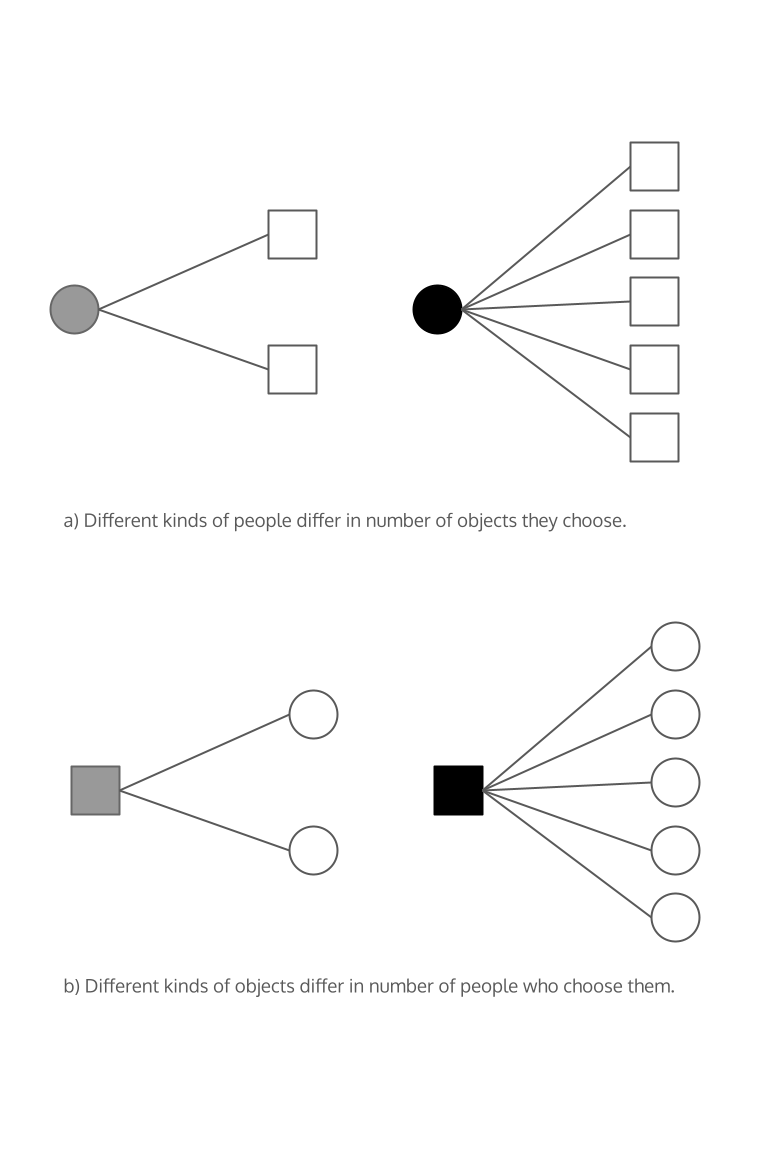
\includegraphics[width=0.8\linewidth]{Figs/local-struct1.png}
    \caption{Local structural neighborhoods of omnivorousness and popularity.}
    \label{fig:local-struct1}
\end{figure}

\newpage

\begin{figure}
    \centering
    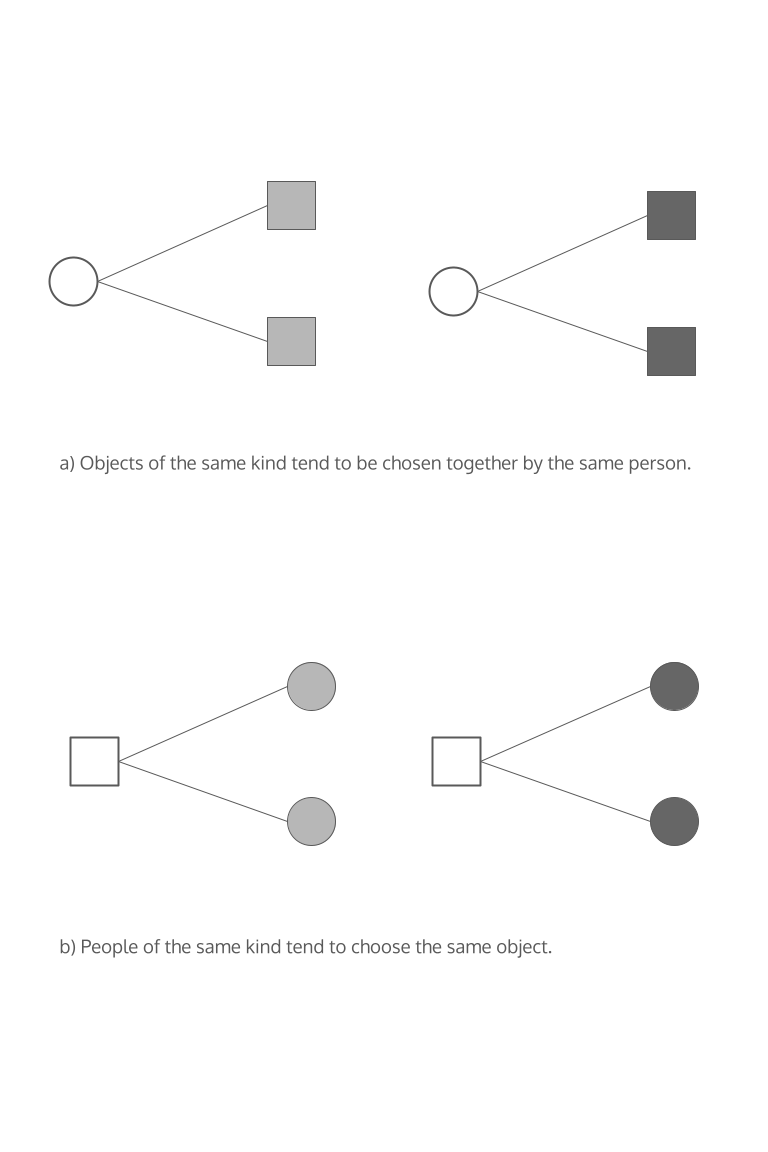
\includegraphics[width=0.8\linewidth]{Figs/local-struct2.png}
    \caption{Local structural neighborhoods of correlated choices based on categorical similarity.}
    \label{fig:local-struct2}
\end{figure}

\newpage

\begin{figure}
    \centering
    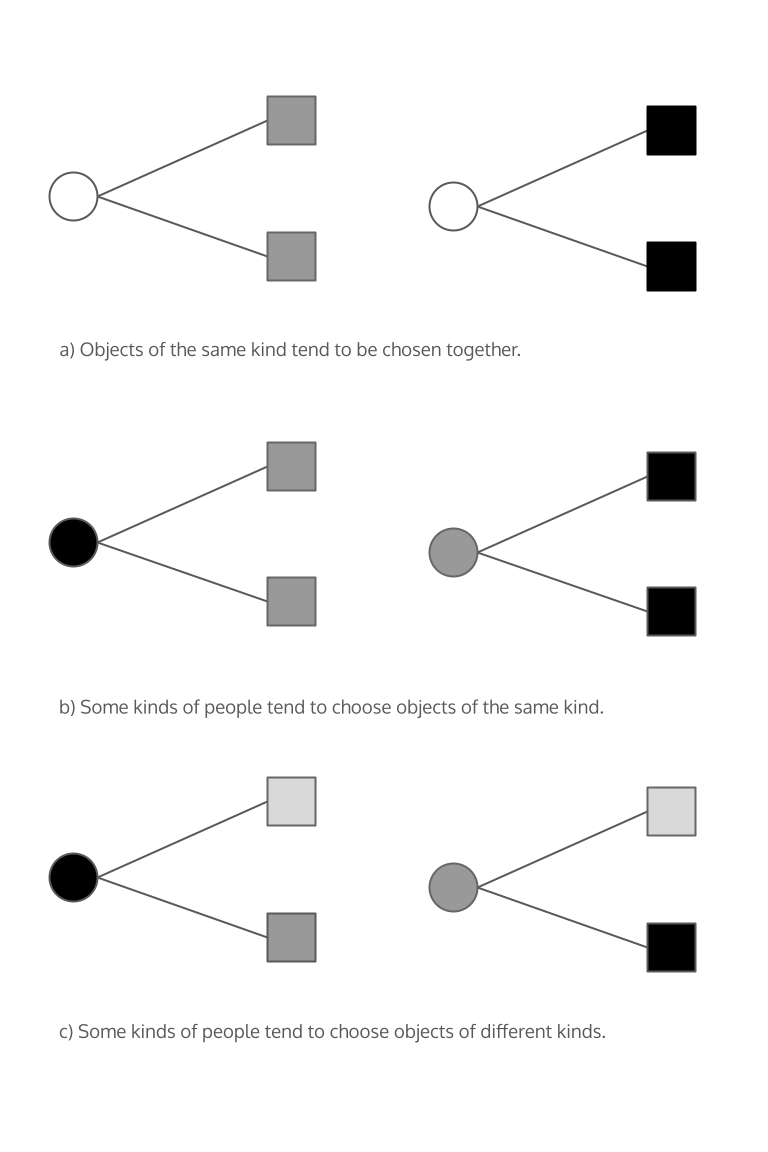
\includegraphics[width=0.8\linewidth]{Figs/local-struct3.png}
    \caption{Local structural neighborhoods of triadic configurations featuring one person and two cultural objects.}
    \label{fig:local-struct3}
\end{figure}



\end{document}

\endinput
%%
%% End of file `elsarticle-template-harv.tex'.
